\documentclass[12pt]{article}
\usepackage{amsmath}
\usepackage{amssymb}
\usepackage{setspace}
\usepackage{graphicx}
\usepackage[margin=1in]{geometry}
\newcommand{\del}{\nabla}
\doublespacing
\begin{document}

\title{Nonlinear Analysis of VR Synchronization}
\author{Howon Lee}
\maketitle

\section{Abstract}
There exists a literature dealing with time series analysis in the nonlinear sciences in the case of synchronization, or the adjustment of rhythms of oscillating objects to coincide with each other due to weak interaction. We attempt many of these methods in analyzing an instance of the phenomenon of interpersonal synchrony in a virtual environment. We also propose a mapping from time series to networks with a deterministic inverse, useful for exploratory analysis.

%%% acknowledgements go here

%%% target is JB, ASW, SG, each of them at once
%%% examples should abound, and should be explicated

\section{Introduction}

Before defining what we mean by synchronization in this context, we note that there exists a long history of the study of synchronization outside of social science. Synchronization was first reported in physical systems by Huygens in 1665. He saw that two pendulum clocks in the boat that he was testing the clocks in were mysteriously ticking in unison, and found that the cause was a support beam which connected the clocks, which moved imperceptibly and therefore maintained the synchronization\cite{huygens}.

Centuries later, the physical and biological systems which were later found to synchronize include mechanical rotators, lasers, fireflies emitting synchronous patterns of light, synchronous contraction of heart cells, synchronization of human circadian rhythm to a solar light cycle, and synchronous interaction of human beings\cite{syncreview}, \cite{physsync}.

Now, we should define the terms. Interpersonal synchrony is defined in the social science literature as individuals' termporal coordination during social interaction\cite{socialsync}. In the physical sciences, synchronization is defined as an adjustment of rhythms of oscillating objects due to weak interaction, with generalizations possible for chaotic systems, which depend upon a phase of the chaotic system existing\cite{physsync}.

Although social synchrony is one of many other synchronies, many of which do not necessarily serve a function of any kind, it is observed that social synchrony serves a function in human social groups. There exists evidence that synchronization acts as a cooperation-enducing mechanism\cite{coop}, that it acts to induce rapport\cite{rapport}, and that it in actuality, independent of its effect on rapport, enhances the ability to pursue joint goals in tandem for those who are synchronized\cite{goals}. This suggests immediately that it must be measured in a systematic way, to study phenomena of that kind.

In the beginning of the social synchronization literature, most psychologists did not use the then-developing automated signals processing techniques for the detection and measurement of synchronization, instead using manual methods to detect and rate the presence or absence of synchronization, with trained raters and validated measuring systems\cite{manual}. Although these measurements have been validated\cite{manualval}, they depend upon human raters and therefore are less replicable and less convenient than automated systems.

Given that the signals created by an individual during social interaction have a phase, and social interaction can be construed as a weak interaction between the two individual systems, it should be clear that the definition of interpersonal synchrony given in the social psychological literature is a subset of the definition given in the physics literature. This has often been noted\cite{socialsync}, and has therefore spawned a cross-disciplinary field wherein signals processing techniques are used to measure interpersonal synchrony.

As a specific instance of a domain where signals processing techniques are used, a large problem in synchronization is the definition of the signal itself and its extraction from observations of social interaction. To this end, many methods have been used, including extraction of coordination of movement features and speech features, movement of single and dyadic body parts, image processing techniques and video tracking techniques. %%% cite a bunch of stuff from delaherche cohen paper and my own lit stuff

An important analogy exists between the collection of time series data about the physiology of the body in order to assess synchrony and the collection of time series data about the body in order to assess health. Indeed, there exists a literature on the synchronization properties and the time series analysis of heart rate variability which we have derived much inspiration from, not necessarily in the usage of correlational metrics, for which there is a literature dealing in social synchronization, but more sophisticated metrics for which there is not such a literature\cite{hrv1}\cite{hrv2}. The essential premise is that we treat social synchronization as an instance of an abstract problem of physical synchronization, which justifies using measures used by other physiological measurements.

------------ vr benefits: experimental control versus ecological validity: but you don't have to choose between the tool, you can escape the lab in a controlled setting with virutal reality. naturalistic vision of vistas and scenes, naturalistic ability to interact socially, although I think this condition was mixed media. really great data collection\cite{blascovich}
%%%%%%%%%%%%%%%%%%%%%%%%%%%%%%%%
%%%%%%%%%%%%%%%%%%%%%%%%%%%%%%%%

This project will attempt to use some of the already existing tools for the analysis of time series data on VR time series data, as well as apply some tools which have not previously been used to analyze synchronization in VR time series data of social synchronization in a virtual world.
--- summary of what exists, talk only about the fact that they exist, as a preliminary summary of the essay. we will go deeper and actually formal with this one. correlation, MI in physics, spectral methods, analytic signal, graph analysis
%%%%%%%%%%%%%%%%%%%%%%%%%%%%%%%%
%%%%%%%%%%%%%%%%%%%%%%%%%%%%%%%%

\subsection{Justification for Nonlinear Measures}
%%% why it's different than other approaches to measuring interactional synchrony

--- there's a big correlational and phase coherence literature. talk about it, why it exists.

--- there's a big machine learning literature, basically talk the book on the synchronization stuff

--- there's the large sensorimotor literature, they've never used nonlinear stuff.

--- note the physics kids distinction of simple and more complex synchronizations: phase and amplitude synchronizations, those apply to the person as well. so we should not ignore nonlinear measures.

One might wonder why the existing methods of measurement of synchronization do not already serve for the purpose of measuring synchronization of body movements in VR. They do not serve for the same reasons that they do not serve in physical time series. That is, they are fundamentally \emph{linear} measures of the relation that they have to each other, meaning that measuring only correlation implicitly puts in the assumption that an affine transform relates the two signals to each other. It is possible to learn about higher order dependences if correlations of higher moments are used, but this becomes rapidly time-consuming very quickly\cite{pompe}.

\begin{figure}\label{fig:nonlinearity}
  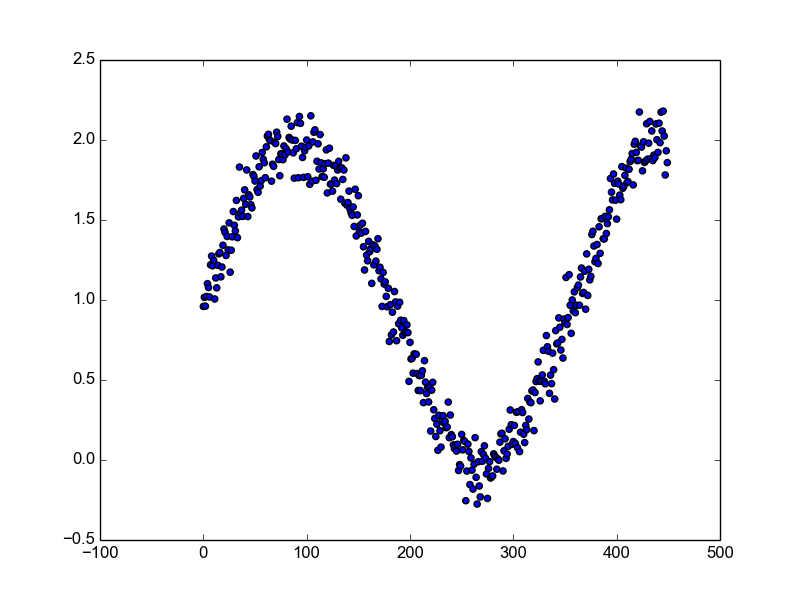
\includegraphics[scale=0.5]{mi_ex}
  \caption{Example of simple nonlinear relation between two variables}
\end{figure}

One example which should help develop a theoretical intuition about nonlinearity and synchronization is the sine wave relation example. Consider the figure \ref{fig:nonlinearity}. According to a linear correlation measure, taking the whole domain of $x$ into account at once, the two variables $x$ and $y$ cannot disprove the null hypothesis of independence ($p=0.45$), but by inspection, one can say that actually $y = sin(x) + \epsilon$, where $\epsilon$ is a small amount of Gaussian noise. But nonlinear measures \emph{will} take this nonlinear relation into account. For example, mutual information will say that the mutual information between the two variables $x$ and $y$ is 7.5 bits, which indicates that the variables determine each other to a great degree.

We will claim that relations of this sort are common in physiological data of all kinds. %%%% recapitulate those arguments from physiological data, cite a lot of the physiological data literature. If neuronal signals are nonlinear and can be related in an MI sort of way, why not the physiological movements which are caused by those neuronal signals?

\subsection{Data Description}

--- This is the place where we will describe the data we got, the ad hoc analyses made previously to fold in the data into small number of dimensions. Discuss the data incompletion problem.

--- Why the dimensionality reduction? we suffer from curse of dimensionality
%%%%%%%%%%%%%%%%%%%%%%%%%%%%%%%%%%%%%%%%%%%%%%
%%% to do this analysis, we will use the data of a previously published study (as won et al), where synchronization was measured in 50 or so dyads on a kinect.
%%%%%%%%%%%%%%%%%%%%%%%%%%%%%%%%%%%%%%%%%%%%%%

\section{Time Domain Analysis}

\subsection{Correlation Analysis}

%% how Andrea did it, basically: 400 windows, Pearson's r. What is correlational analysis, really. What can it do. With a picture. What is autocorrelation. What is cross-correlation.
%% add the MC plot of correlation. add the summary plot of correlation over the entire dataset.
%% describe what a poincare plot is. put an example one in. describe our poincare plot summary measure, and put the summary in
%% describe and add the cornettos

One analysis commonly used with relaxation oscillators like ECG data is the Poincare map, not to be confused with the Poincare plot. However, because there are not clear demarcations as to where each oscillation is, the Poincare map is less suited to this dataset and will not be used\cite{poincaremap}

\subsection{Mutual Information Analysis}

In order to introduce mutual information, we must introduce Shannon information and Shannon entropy.

Shannon information is defined on a measurement drawn from some set (let the set be discrete, $X \in {1 ... n}$, for ease of notation: there exist continuous analogues). Given that measurement from some set, the Shannon information in bits is defined as:

$$ -\log_2 P_X(i) $$

where $P_X(i)$ is the probability that a measurement will find the system in state $i$. That is, a lower probability answer is more surprising, and therefore more information is found in it.

Shannon entropy, denoted $H(X)$ is defined on a data stream (a measurement stream) $X$. It is the average amount of information contained in every message received, and so is also measured in bits. An easy intuition about entropy can be gained by noting that a \emph{fair} coin flipping process is the most entropic possible coin flip, because we are most surprised by it. Formally, entropy is:

$$H(X) = -\sum_i P_X(i) \log_2 P_X(i)$$

Information and entropy are also defined on joint probability distributions in an analogous way. The information of a joint probability distribution on variables $X$ and $Y$ is:

$$ -\log_2 P_{XY}(i, j) $$

And the entropy, therefore, is:

$$H(X, Y) = -\sum_i \sum_j P_{XY}(i, j) log_2 P_{XY}(i, j)$$

Now, if we sample two random variables simultaneously, the relationship has a quantity defined upon it which is called the \emph{mutual information}. Because it is defined on the relation, it has an auto-mutual information variant and a cross-mutual information variant, like correlation does. However, mutual information measures something different, which is the \emph{information which one of the random variables gives me about the other random variable}. It is defined as:

$$I(X, Y) = H(X) + H(Y) - H(X, Y)$$

And one sees that this quantity is symmetric with respect to $X$ and $Y$.

\subsubsection{AMI and CMI}

Auto-mutual information (AMI) and cross mutual information(CMI) are the mutual information analogues to autocorrelation and cross-correlation. They have the same advantages over the correlation variants as mutual information itself has to correlation. Therefore, they are better measurements for synchronization.

------ actual content of Mutual information analysis goes here.
%%%%%%%%%%%%%%%%%%%%%%%%%%%
%%%%%%%%%%%%%%%%%%%%%%%%%%%
%%%%%%%%%%%%%%%%%%%%%%%%%%%

\section{Frequency Domain Analysis}

There is more than one way to represent time series data, even given only the data itself and not any underlying function that generates it. The most important alternate representation is the frequency domain representation, which is taken in finite data with the discrete Fourier transform. Later, we will show the use of the frequency representation in re-representing our data so that it shows a numerical current state of the phase, using the related Hilbert transform.

The frequency domain represents data in terms of the linear combination of simple sine and cosine waves: the analogy often used is that of a chord being hit on a piano, which can be represented with its time domain signal but can also be represented as the amplitude of the individual notes within the chord, which presents a better decomposition of the sound in and of itself. Likewise, we can attempt to decompose our time domain signals into the frequencies of the sinusoids which make it up.

The discrete fourier transform is an essential tool for the further analyses below. It converts a finite discrete sample from the time to the frequency domain in a computable and fast way.

---- add back in the math of DFT
---- add back in the coherence measures

%%% short section on math of dft. why is it a _transform_? (aka, show that math). what is power spectrum? what is the relation to the autocorrelation?

%%% other people have used spectral methods.

%%% why use coherence instead of other measures?

\subsection{Hilbert Transform and $\gamma$}

A signal is called an \emph{analytic signal} if it does not have any negative-frequency components. The Hilbert transform is a way to get the analytic \emph{representation} for a signal in the time domain, which throws away the superfluous information which would be in a spectrum of that signal. This allows the expression of the analytic signal in terms of its time-variant magnitude and phase, allowing a study of the phase in an \emph{unwrapped form}\cite{gabor}.

Formally speaking, given that the original signal is $s(t)$, the analytic signal $\zeta$ is:

$$\zeta(t) = s(t) + js_H(t) = A(t)e^{j\phi(t)}$$

$$s_H(t) = \frac{1}{\pi} PV \int_{-\infty}^{\infty} \frac{s(t)}{t - \tau} d\tau$$

$s_H$ is called the Hilbert transform; $PV$ indicates that the integral is a Cauchy principal value integral. The Hilbert transform is thus formally equivalent to convolution of $s(t)$ with $\frac{1}{\pi t}$, so it can easily be calculated from the fast Fourier transform.

--- finish the Hilbert transform, add the justification (you can take out the amplitude entirely as a factor, whereas coherence and that sort of thing ends up not doing this).
--- add pretty pictures of unwrapped hilbert transform, and the description of the gammadifference measures
--- -then- add the gamma results and the hilbert transform results themselves
%%%%%%%%%%%%%%%%%%%%%%%%%%%%%%
%%%%%%%%%%%%%%%%%%%%%%%%%%%%%%
%%%%%%%%%%%%%%%%%%%%%%%%%%%%%%

\begin{thebibliography}{}
  \bibitem{huygens}
  \bibitem{syncreview}
  \bibitem{physsync}
  \bibitem{socialsync}
  \bibitem{coop}
  \bibitem{rapport}
  \bibitem{goals}
  \bibitem{campanharo}
  \bibitem{pushdown}
  \bibitem{multigraph}
  \bibitem{manual}
  \bibitem{manualval}
  \bibitem{blascovich}
  \bibitem{pompe}
  \bibitem{poincaremap}
  \bibitem{hrv1}
  \bibitem{hrv2}
  \bibitem{gabor}
\end{thebibliography}

\end{document}
